\documentclass[11pt, a4paper]{article}

\usepackage[top=2cm, bottom=2cm, left=2.5cm, right=2cm]{geometry}
\usepackage{fontspec}
\usepackage{amsmath, amssymb}
\usepackage{booktabs}
\usepackage{tabularx}
\usepackage{graphicx}
\usepackage{float}
\usepackage{xcolor}
\usepackage{hyperref}
\usepackage{xurl}
\usepackage{parskip}
\usepackage{listings}
\usepackage{microtype}
\usepackage{caption}
\usepackage{enumitem}
\usepackage{tikz}
\usetikzlibrary{positioning, arrows.meta}

\setmainfont{Times New Roman}
\graphicspath{{images/}}
\emergencystretch=10em

\hypersetup{
    colorlinks=true,
    linkcolor=blue!70!black,
    citecolor=blue!70!black,
    urlcolor=blue!70!black,
    pdftitle={Assignment 07 - 5-layer RNN and LSTM: PyTorch and Keras},
    pdfauthor={Luu Anh Dung}
}

\lstset{
    basicstyle=\footnotesize\ttfamily,
    breaklines=true,
    frame=single,
    backgroundcolor=\color{gray!10},
    columns=fullflexible
}

\newcommand{\run}[1]{\texttt{#1}}
\newcommand{\why}[1]{\textbf{Why.} #1}
\setlist{itemsep=2pt, topsep=4pt}

\begin{document}

% ---------------------------------------------------------
% COVER PAGE
% ---------------------------------------------------------
\begin{titlepage}
\begin{center}

\vspace*{0.5cm}

\Large
\textbf{POSTS AND TELECOMMUNICATIONS INSTITUTE OF TECHNOLOGY}\\
\textbf{Faculty of Information Technology}

\vspace{2.0cm}

\Huge
\textbf{Intelligent System Development}\\
\vspace{0.4cm}
\LARGE
\textbf{ASSIGNMENT 07}\\
\vspace{0.6cm}
\Large
\textbf{5-Layer RNN and LSTM as Compositions of Elementary Functions:\\
PyTorch and Keras on Review Sentiment and Stock Volatility}

\vspace{1.2cm}

\vfill

\normalsize
\begin{tabular}{rl}
\textbf{Instructor / Lecturer:} & Assoc. Prof. Dinh Que Tran, Ph.D. \\
\textbf{Email:} & quetd@ptit.edu.vn, tdque@yahoo.com \\[0.8cm]
\textbf{Student Name:} & Lưu Anh Dũng \\
\textbf{Student ID:} & B23DCDK036 \\
\textbf{Semester:} & I.2025 -- 2026 \\
\textbf{Submission:} & Individual Project \\
\end{tabular}

\vfill

\textbf{Hanoi, 2026}

\vspace{0.5cm}

\end{center}
\end{titlepage}

\tableofcontents
\newpage

% =====================================================================
\section*{Summary}
\addcontentsline{toc}{section}{Summary}
% =====================================================================

This report builds a \textbf{5-layer recurrent neural network (RNN)} and a \textbf{5-layer LSTM} from five elementary
functions (matrix product, addition, $\tanh$, sigmoid and element-wise product), checks that PyTorch and Keras compute
exactly these compositions, and compares the two architectures on two Kaggle datasets of about 100\,MB each:
\textbf{EC}, 148{,}124 e-commerce review comments (Amazon unlocked mobile phones, sentiment classification), and
\textbf{ST}, daily prices of 145 S\&P~500 stocks over 15 years (next-day volatility forecasting).
Two datasets $\times$ two architectures $\times$ two frameworks give 8 runs, all with the same data, protocol and
initialisation. Run IDs have the form \run{<dataset>-<framework>-<model>}, e.g.\ \run{EC-PT-LSTM}.

\begin{table}[H]
\centering
\caption{RNN against LSTM on the test sets. Score: macro F1 (EC) and out-of-sample $R^2$ against the train mean (ST);
$\Delta$ = LSTM $-$ RNN; time = median seconds per epoch on CPU.}
\label{tab:summary}
\small
\resizebox{\textwidth}{!}{\begin{tabular}{llrrrrr}
\toprule
Run & main metric & value & second metric & params & s/epoch & train time (s) \\
\midrule
\run{EC-TF-RNN} & macro-F1 & 0.614 & acc. 0.829 & 760{,}451 & 69.7 & 286 \\
\run{EC-PT-RNN} & macro-F1 & 0.605 & acc. 0.830 & 760{,}771 & 143.4 & 566 \\
\run{EC-TF-LSTM} & macro-F1 & 0.682 & acc. 0.834 & 881{,}219 & 278.4 & 1127 \\
\run{EC-PT-LSTM} & macro-F1 & 0.695 & acc. 0.829 & 882{,}499 & 188.2 & 1126 \\
\midrule
\run{ST-TF-RNN} & RMSE (\%) & 0.6849 & $R^2$ 0.320 & 9{,}569 & 20.2 & 87 \\
\run{ST-PT-RNN} & RMSE (\%) & 0.6956 & $R^2$ 0.299 & 9{,}729 & 31.1 & 127 \\
\run{ST-TF-LSTM} & RMSE (\%) & 0.6788 & $R^2$ 0.332 & 38{,}177 & 86.5 & 362 \\
\run{ST-PT-LSTM} & RMSE (\%) & 0.6828 & $R^2$ 0.324 & 38{,}817 & 66.3 & 264 \\
\bottomrule
\end{tabular}}
\end{table}

\textbf{Key findings}
\begin{enumerate}
\item \textbf{The frameworks compute the written compositions.} A NumPy implementation written from the formulas matches
  PyTorch and Keras to $\le 2\cdot10^{-7}$ for both cells, and the hand-counted parameters match the framework counts exactly.
\item \textbf{The gradient explains the architecture.} In a freshly initialised 5-layer RNN, the first step of the first
  layer receives $8.7\cdot10^{-11}$ of the gradient at the output after 50 steps; an LSTM with forget-gate bias 1 receives $4.5\cdot10^{-4}$.
\item \textbf{EC: the LSTM wins, most on long reviews.} It beats the RNN by 0.8--1.8 points of macro F1 and 0.9--2.7 points of
  F1 on the negative class, and the gap is largest on reviews longer than 100 words. A TF-IDF + logistic regression
  baseline (F1 0.930) is still better than both, because the sentiment here is carried by single words.
\item \textbf{ST: both networks double the classical baseline, the LSTM only slightly more.} $R^2_{\text{oos}}\approx0.09$
  against 0.044 for the 20-day mean; LSTM $-$ RNN is only $+0.004$ to $+0.009$, because the useful memory of volatility is a few weeks.
\item \textbf{Cost.} The LSTM has 4$\times$ the recurrent parameters and takes 1.8--4.8$\times$ longer per epoch.
  Keras and PyTorch agree to within 0.016 on every metric.
\end{enumerate}

% =====================================================================
\section{Introduction}
% =====================================================================

A recurrent network reads a sequence one step at a time and carries a hidden state from step to step, so the same
model can read a review of 10 words or one of 100 words, or a window of 60 trading days. Stacking several recurrent
layers lets higher layers work on more abstract summaries, but a plain RNN learns poorly from inputs far in the past:
its gradient is multiplied by a shrinking factor at every step and every layer. The LSTM adds a gated memory cell whose
update is additive, so the gradient can travel back many steps. Following the lecturer's view that
\emph{a neural architecture is a structured composition of functions} and that
\emph{a new architecture is an old one plus a mechanism that addresses a limitation}, this report writes both networks as
compositions of elementary functions, explains why each piece is there, and then measures whether the LSTM's mechanism
pays off on real data.

\textbf{Brief.} (R1) Two datasets: user comments from e-commerce and a Kaggle stock dataset, of moderate size
(about 100\,MB each). (R2) The structure of a 5-layer RNN as a composition of elementary functions, with explanation.
(R3) The same for the LSTM. (R4) Code in PyTorch and Keras. (R5) Run and evaluate. (R6) Compare LSTM and RNN on both
datasets. (R7) Notebooks and report.

\begin{table}[H]
\centering
\caption{Where each requirement is answered.}
\small
\begin{tabularx}{\textwidth}{llX}
\toprule
\# & Requirement & Sections and evidence \\
\midrule
R1 & Datasets & \S\ref{sec:data}: selection, size, cleaning, exploratory figures \\
R2 & 5-layer RNN structure & \S\ref{sec:functions}, \S\ref{sec:rnn}: formulas, unrolled grid, numeric example, parameters, gradient map \\
R3 & 5-layer LSTM structure & \S\ref{sec:lstm}: gates, cell path, parameters, gradient flow \\
R4 & PyTorch and Keras code & \S\ref{sec:impl}: listings, weight mapping, verification \\
R5 & Run and evaluate & \S\ref{sec:setup}--\S\ref{sec:st}: protocol, baselines, results, curves, error analysis \\
R6 & Compare LSTM and RNN & \S\ref{sec:compare}: accuracy, parameters, time, behaviour \\
R7 & Notebooks and report & Appendix~\ref{app:repro} \\
\bottomrule
\end{tabularx}
\end{table}

The work is in three notebooks: \texttt{00\_rnn\_lstm\_concepts.ipynb} (\S2--\S5), \texttt{ec\_reviews.ipynb} and
\texttt{st\_stocks.ipynb} (\S5--\S10). All numbers in this report are taken from their executed outputs.

% =====================================================================
\section{Elementary Functions and Composition}
\label{sec:functions}
% =====================================================================

Both networks use only the five functions of Table~\ref{tab:elem}. Vectors are row vectors, so a layer is written $xW$.

\begin{table}[H]
\centering
\caption{The elementary functions, with the tiny example computed in the concepts notebook.}
\label{tab:elem}
\small
\begin{tabularx}{\textwidth}{lllX}
\toprule
Function & Formula & Example & Role \\
\midrule
matrix product & $(xW)_j=\sum_i x_iW_{ij}$ & $(1,2)\begin{pmatrix}1&0\\3&1\end{pmatrix}=(7,2)$ & every unit sees every input, each with its own weight \\
addition & $a+b$ & $(7,2)+(0.5,-1)=(7.5,1)$ & merges the new input with the memory \\
$\tanh$ & $\frac{e^z-e^{-z}}{e^z+e^{-z}}\in(-1,1)$ & $\tanh(0.5)=0.4621$ & activation of the RNN and of the LSTM candidate \\
sigmoid & $\sigma(z)=\frac1{1+e^{-z}}\in(0,1)$ & $\sigma(2)=0.8808$ & gate: the fraction of a signal let through \\
element-wise product & $(a\odot b)_i=a_ib_i$ & $(0.9,0.1)\odot(4,4)=(3.6,0.4)$ & applies a gate to each unit separately \\
\bottomrule
\end{tabularx}
\end{table}

Their derivatives decide how well a gradient passes through them: $\tanh'(z)=1-\tanh^2z\le1$ and
$\sigma'(z)=\sigma(1-\sigma)\le0.25$. A saturated unit passes almost nothing: $\tanh'(3)=1-0.9951^2=0.0099$.

\why{}
\begin{itemize}
\item \emph{A nonlinearity is required.} Two linear layers collapse into one, $(xW_1)W_2=x(W_1W_2)$, so five layers
  without $\tanh$ would be a single matrix and could only draw straight decision boundaries.
\item \emph{$\tanh$ rather than ReLU in a recurrence.} The same recurrent matrix is applied at every step. ReLU has no
  upper bound, so a matrix that scales the state by 1.1 makes it $1.1^{50}\approx117$ times larger after 50 steps;
  $\tanh$ brings every step back into $(-1,1)$ and is zero-centred, so states can be positive or negative.
\item \emph{Sigmoid for gates.} A gate is a fraction between ``block'' (0) and ``pass'' (1), exactly the range of $\sigma$;
  $\tanh$ cannot serve as a gate because it takes negative values.
\item \emph{Element-wise product.} A gate decides for each unit separately (keep unit 1, forget unit 2), so it multiplies
  position by position, not through a full matrix.
\end{itemize}

% =====================================================================
\section{Structure of the 5-Layer RNN}
\label{sec:rnn}
% =====================================================================

\subsection{One cell: three elementary functions}

At step $t$ the cell combines the new input $x_t\in\mathbb{R}^F$ with its previous state $h_{t-1}\in\mathbb{R}^H$:
\begin{equation}
h_t=\tanh\big(\underbrace{x_tW_x}_{\text{matmul}}+\underbrace{h_{t-1}W_h}_{\text{matmul}}+b\big),\qquad h_0=0,
\qquad\text{i.e.}\quad h_t=\tanh\circ\operatorname{add}(x_tW_x,\;h_{t-1}W_h,\;b).
\end{equation}
\textbf{Example} ($F=H=2$, weights from the notebook): $x_1=(1,0)$ gives the pre-activation $a=(0.5,-0.2)$ and
$h_1=\tanh(a)=(0.4621,-0.1974)$; at $t=2$, $a=(1.1357,0.2756)$ and $h_2=(0.8130,0.2689)$, so $h_2$ depends on $x_1$ through $h_1W_h$.

\why{} $x_tW_x$ is \emph{what is new} and $h_{t-1}W_h$ is \emph{what was seen before}; adding them makes $h_t$ a running
summary of $x_1,\dots,x_t$. $h_0=0$ because nothing has been seen yet. The same $W_x,W_h,b$ are used at every step
(\textbf{weight sharing}) because the rule for reading a word should not depend on its position: ``not good'' means the
same at word 3 and at word 80, a 2\,\% price drop the same on any day. Sharing also fixes the model size: one $W_h$
serves sequences of any length. Unrolled, $h_3=\tanh(x_3W_x+\tanh(x_2W_x+\tanh(x_1W_x+b)W_h+b)W_h+b)$: the first input
reaches the output only through nested $W_h$ and $\tanh$, which is the origin of the gradient problem in \S\ref{sec:grad}.

\subsection{Stacking five layers}

Layer 1 reads the input sequence; layer $l$ reads the hidden states of layer $l-1$ as its input sequence:
\begin{equation}
h^{(1)}_t=\tanh\big(x_tW^{(1)}_x+h^{(1)}_{t-1}W^{(1)}_h+b^{(1)}\big),\qquad
h^{(l)}_t=\tanh\big(h^{(l-1)}_tW^{(l)}_x+h^{(l)}_{t-1}W^{(l)}_h+b^{(l)}\big),\ l=2,\dots,5.
\end{equation}
The prediction uses the top layer at the last step, $\hat y=g\big(h^{(5)}_TW_y+b_y\big)$. If $f^{(l)}$ denotes the map
from a sequence to the sequence of layer-$l$ states, the whole network is one composition:
\begin{equation}
\hat y = g\circ\operatorname{last}\circ f^{(5)}\circ f^{(4)}\circ f^{(3)}\circ f^{(2)}\circ f^{(1)}\,(x_1,\dots,x_T),
\end{equation}
where each $f^{(l)}$ is $T$ repetitions of matmul $\to$ add $\to\tanh$. Figure~\ref{fig:grid} shows the resulting grid.

\begin{figure}[H]
\centering
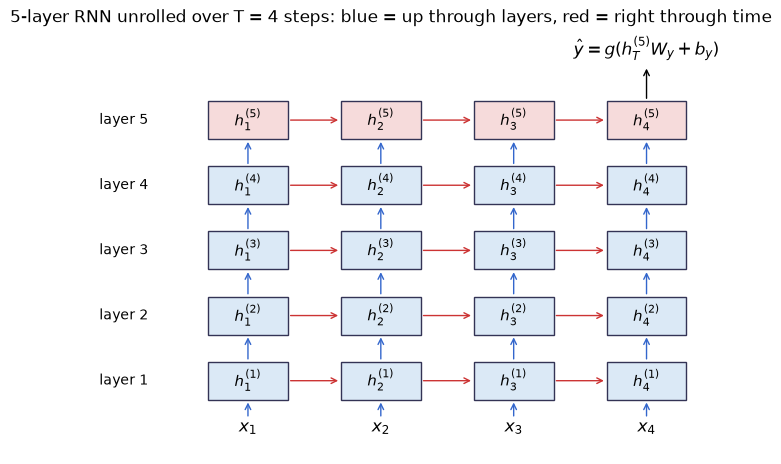
\includegraphics[width=0.72\textwidth]{C_grid.png}
\caption{The 5-layer RNN unrolled over $T=4$ steps. Information moves up through the layers (blue) at the same step and
right through time (red) within a layer; only $h^{(5)}_T$ feeds the output.}
\label{fig:grid}
\end{figure}

\why{}
\begin{itemize}
\item \emph{Stack layers.} Each layer re-reads the sequence produced by the layer below, so higher layers summarise at a
  higher level: on reviews, single words (``good''), then phrases (``not good''), then the verdict; on stocks, one day's
  move, then patterns over weeks such as calm or turbulent periods. One layer could in principle do the same with many
  more units; depth reuses the features already built below.
\item \emph{Only the last step of the top layer.} Through the recurrence $h^{(5)}_T$ depends on every input, so it already
  summarises the sequence, and both tasks need one answer per sequence.
\item \emph{The output function $g$.} For sentiment $g=\sigma$ gives a probability, trained with binary cross-entropy;
  for volatility $g$ is the identity, trained with squared error, because squashing would cap the forecast.
\end{itemize}

\textbf{Shapes} through the two dataset models for a batch of 256 (Table~\ref{tab:shapes}): the hidden size stays $H$ in
every layer, and only the last layer drops the time axis.

\begin{table}[H]
\centering
\caption{Tensor shapes (batch 256). EC uses a word embedding before layer 1.}
\label{tab:shapes}
\small
\begin{tabular}{lll}
\toprule
Stage & EC (reviews) & ST (stocks) \\
\midrule
input & $(256,100)$ word ids & $(256,60,4)$ features \\
embedding $20{,}000\times64$ & $(256,100,64)$ & -- \\
layers 1--4 (all steps) & $(256,100,64)$ & $(256,60,32)$ \\
layer 5, last step $h^{(5)}_T$ & $(256,64)$ & $(256,32)$ \\
head & $(256,1)$, $\sigma$ & $(256,1)$, identity \\
\bottomrule
\end{tabular}
\end{table}

\subsection{Parameters}
\label{sec:rnnparams}

Layer 1 maps $F\to H$ and layers 2--5 map $H\to H$:
\begin{equation}
N_{\text{RNN}}=\underbrace{FH+H^2+H}_{\text{layer 1}}+\underbrace{(L-1)(H^2+H^2+H)}_{\text{layers 2--5}}+\underbrace{H+1}_{\text{head}}.
\end{equation}
\why{} $W_x$ is $F\times H$ because each of the $H$ units has one weight per input; above layer 1 the inputs are the $H$
states of the layer below. $W_h$ is $H\times H$ because each unit looks at the previous state of all $H$ units of its
layer, itself included. $b$ is one number per unit. The count does not depend on $T$ (weight sharing).
PyTorch stores two bias vectors per layer (\texttt{bias\_ih}, \texttt{bias\_hh}, a cuDNN convention); only their sum enters
the formula, so it has $L\cdot H$ more numbers but computes the same function.

\begin{table}[H]
\centering
\caption{Parameters: hand formula (Keras, one bias) against the framework counts.}
\label{tab:params}
\small
\begin{tabular}{lrrrr}
\toprule
Model & Formula & Keras & PyTorch & PyTorch $-$ formula \\
\midrule
toy RNN ($F=3,H=4$) & $32+4\cdot36+5=181$ & 181 & 201 & $L\cdot H=20$ \\
toy LSTM ($F=3,H=4$) & $4\cdot32+16\cdot36+5=709$ & 709 & 789 & $4LH=80$ \\
\run{EC-*-RNN} (incl.\ embedding) & 1{,}321{,}345 & 1{,}321{,}345 & 1{,}321{,}665 & 320 \\
\run{EC-*-LSTM} (incl.\ embedding) & 1{,}445{,}185 & 1{,}445{,}185 & 1{,}446{,}465 & 1{,}280 \\
\run{ST-*-RNN} ($F=4,H=32$) & 9{,}537 & 9{,}537 & 9{,}697 & 160 \\
\run{ST-*-LSTM} & 38{,}049 & 38{,}049 & 38{,}689 & 640 \\
\bottomrule
\end{tabular}
\end{table}

The dataset notebooks assert these counts before training, so a model that does not match the formula cannot run.

\subsection{Why depth and length hurt: the gradient}
\label{sec:grad}

Training needs $\partial\mathcal{L}/\partial h^{(l)}_t$ for every layer and step. With $h_t=\tanh(a_t)$ and
$a_t=x_tW_x+h_{t-1}W_h+b$, the chain rule gives
\begin{equation}
\frac{\partial h_t}{\partial h_{t-1}}=\underbrace{\operatorname{diag}(1-h_t^2)}_{\tanh'}\,W_h^\top,\qquad
\frac{\partial h_T}{\partial h_t}=\prod_{k=t+1}^{T}\operatorname{diag}(1-h_k^2)\,W_h^\top,
\end{equation}
and going down one layer multiplies by $\operatorname{diag}(1-h^2)\,W_x^\top$.

\why{} Every factor contains $1-h^2\le1$. If each step multiplies the signal by 0.6, after 50 steps it is
$0.6^{50}\approx8\cdot10^{-12}$ (\textbf{vanishing}); if by 1.2, it is $1.2^{50}\approx9{,}100$ (\textbf{exploding}).
The update of the weights that read the first words is proportional to this gradient, so with $10^{-11}$ the first words
teach the model nothing and the RNN effectively learns from the last few steps. Explosion is handled by gradient
clipping (clip-norm 1 in all runs); vanishing cannot be clipped away and needs a different cell.
Figure~\ref{fig:grad} measures this on a freshly initialised 5-layer RNN ($T=50$, $H=32$) with the loss on the top-right
state only: step 1 of layer 1 receives $8.7\cdot10^{-11}$ of the gradient.

% =====================================================================
\section{Structure of the 5-Layer LSTM}
\label{sec:lstm}
% =====================================================================

\subsection{The cell: gates from the same functions}

The LSTM keeps the RNN's limitation in view and adds one mechanism: a second state, the \textbf{cell} $c_t$, updated by
addition and controlled by three gates (Table~\ref{tab:gates}, Figure~\ref{fig:lstmcell}). Each gate is the RNN formula with
a sigmoid instead of $\tanh$.

\begin{table}[H]
\centering
\caption{One LSTM step. $W_\ast$ act on $x_t$, $U_\ast$ on $h_{t-1}$.}
\label{tab:gates}
\small
\begin{tabularx}{\textwidth}{llX}
\toprule
Piece & Formula & Role and why \\
\midrule
input gate & $i_t=\sigma(x_tW_i+h_{t-1}U_i+b_i)$ & how much new content to write \\
forget gate & $f_t=\sigma(x_tW_f+h_{t-1}U_f+b_f)$ & how much of the old cell to keep \\
candidate & $g_t=\tanh(x_tW_g+h_{t-1}U_g+b_g)$ & new content; signed, so it can push a memory up or down \\
output gate & $o_t=\sigma(x_tW_o+h_{t-1}U_o+b_o)$ & how much of the cell to show \\
cell & $c_t=f_t\odot c_{t-1}+i_t\odot g_t$ & memory, updated by \textbf{addition} \\
hidden & $h_t=o_t\odot\tanh(c_t)$ & output; $\tanh$ bounds the cell, which can grow past 1 \\
\bottomrule
\end{tabularx}
\end{table}

\begin{figure}[H]
\centering
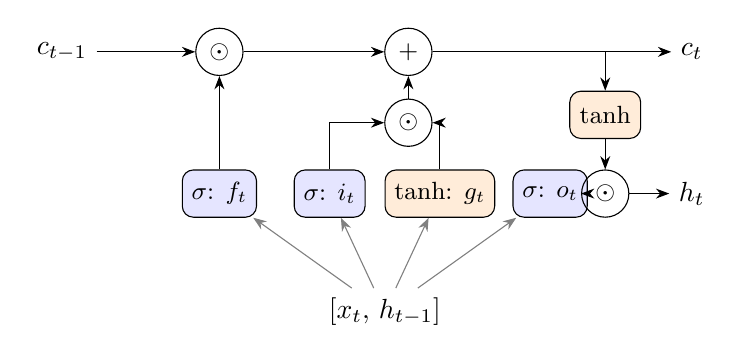
\begin{tikzpicture}[>=Stealth, node distance=1.1cm,
  op/.style={circle, draw, minimum size=6mm, inner sep=0pt, font=\small},
  gate/.style={rectangle, draw, rounded corners, fill=blue!10, minimum width=9mm, minimum height=6mm, font=\small}]
  \node (cin) at (0,2.4) {$c_{t-1}$};
  \node[op] (mulf) at (2,2.4) {$\odot$};
  \node[op] (add) at (4.4,2.4) {$+$};
  \node (cout) at (8,2.4) {$c_t$};
  \node[gate] (f) at (2,0.6) {$\sigma$: $f_t$};
  \node[gate] (i) at (3.4,0.6) {$\sigma$: $i_t$};
  \node[gate, fill=orange!15] (g) at (4.8,0.6) {$\tanh$: $g_t$};
  \node[gate] (o) at (6.2,0.6) {$\sigma$: $o_t$};
  \node[op] (mulig) at (4.4,1.5) {$\odot$};
  \node[gate, fill=orange!15] (tc) at (6.9,1.6) {$\tanh$};
  \node[op] (mulo) at (6.9,0.6) {$\odot$};
  \node (hout) at (8,0.6) {$h_t$};
  \node (in) at (4.1,-0.9) {$[x_t,\,h_{t-1}]$};
  \draw[->] (cin) -- (mulf); \draw[->] (mulf) -- (add); \draw[->] (add) -- (cout);
  \draw[->] (f) -- (mulf);
  \draw[->] (i) |- (mulig); \draw[->] (g) |- (mulig); \draw[->] (mulig) -- (add);
  \draw[->] (add) -| (tc); \draw[->] (tc) -- (mulo); \draw[->] (o) -- (mulo); \draw[->] (mulo) -- (hout);
  \foreach \n in {f,i,g,o} \draw[->, gray] (in) -- (\n);
\end{tikzpicture}
\caption{One LSTM cell. The top line is the cell path: one $\odot$ with $f_t$ and one $+$ per step, no weight matrix and no
squashing; this is what lets the gradient travel back.}
\label{fig:lstmcell}
\end{figure}

\textbf{Example.} $f=0.9$, $c_{t-1}=2.0$, $i=0.5$, $g=0.6$: $c_t=0.9\cdot2.0+0.5\cdot0.6=1.8+0.3=2.1$: 90\,\% of the old
memory is kept and a little new content is added.

\why{}
\begin{itemize}
\item \emph{Gates read $x_t$ and $h_{t-1}$}: the decision to keep or write depends on context; after ``not'' the network
  should treat ``good'' differently, and only $h_{t-1}$ knows that ``not'' came before.
\item \emph{The cell is additive}, so
  $\partial c_t/\partial c_{t-1}=\operatorname{diag}(f_t)$ plus small indirect terms. Over 50 steps with $f=0.97$ the
  factor is $0.97^{50}\approx0.22$, against $0.6^{50}\approx8\cdot10^{-12}$ for the RNN.
\item \emph{$h_t=o_t\odot\tanh(c_t)$}: the output gate lets the cell hold information without showing it until it is
  useful (a word read at step 5 can be released at step 90).
\item \emph{The gates are learned}: training moves $f_t$ towards 1 where memory pays off (a ``but'' that flips a review)
  and towards 0 where the memory should reset.
\end{itemize}

\subsection{Stacking and composition}

Stacking works as for the RNN: layer $l$ reads $h^{(l-1)}_t$, and each layer has its own cell $c^{(l)}_t$:
\begin{equation}
\big(h^{(l)}_t,c^{(l)}_t\big)=\operatorname{LSTM}^{(l)}\big(h^{(l-1)}_t,\,h^{(l)}_{t-1},\,c^{(l)}_{t-1}\big),\qquad
\hat y=g\circ\operatorname{last}\circ F^{(5)}\circ\dots\circ F^{(1)}(x_1,\dots,x_T),
\end{equation}
using matmul, add, $\sigma$, $\tanh$ and $\odot$ only. Both frameworks store the four gates side by side in one matrix of
width $4H$, in the order \textbf{i, f, g, o}, because the four products share their inputs and one large product is faster
than four small ones.

\subsection{Parameters}

\begin{equation}
N_{\text{LSTM}}=4(FH+H^2+H)+4(L-1)(2H^2+H)+H+1 .
\end{equation}
\why{} Each of the four blocks (i, f, g, o) has exactly the shape of one RNN layer; the cell update and $h_t$ only combine
the blocks with $\odot$ and $+$ and add no parameters. Hence 4$\times$ the recurrent part (Table~\ref{tab:params}). On ST
this is the full 4$\times$ (9{,}537 $\to$ 38{,}049); on EC the 1.28\,M-parameter embedding dominates, so the total grows by only 9\,\%.

\subsection{Gradient flow and the forget-gate bias}

\begin{figure}[H]
\centering
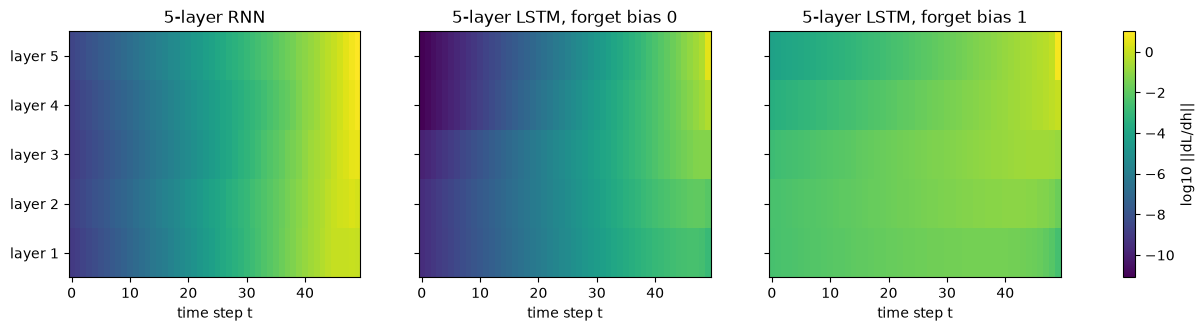
\includegraphics[width=\textwidth]{C_lstm_grad.png}
\caption{$\log_{10}\lVert\partial\mathcal L/\partial h^{(l)}_t\rVert$ for every layer and step of freshly initialised
5-layer networks ($T=50$, $H=32$), loss on the top layer at the last step. Step 1 of layer 1 receives
$8.7\cdot10^{-11}$ (RNN), $9.4\cdot10^{-11}$ (LSTM, forget bias 0) and $4.5\cdot10^{-4}$ (LSTM, forget bias 1).}
\label{fig:grad}
\end{figure}

\why{} At initialisation $f_t\approx\sigma(b_f)$ and the signal through the cell is roughly $f^T$. With bias 0,
$\sigma(0)=0.5$ and $0.5^{50}\approx9\cdot10^{-16}$: the cell starts out forgetting everything and is no better than the RNN.
With bias 1, $\sigma(1)=0.73$ and $0.73^{50}\approx1.6\cdot10^{-7}$, about $10^8$ times larger, so training has a signal to
push $f$ towards 1 where memory is useful. Keras uses bias 1 by default, PyTorch 0; the dataset notebooks set it to 1 in
PyTorch as well so that both frameworks start from the same function.

\begin{table}[H]
\centering
\caption{RNN and LSTM side by side.}
\small
\begin{tabularx}{\textwidth}{lXX}
\toprule
 & 5-layer RNN & 5-layer LSTM \\
\midrule
elementary functions & matmul, add, $\tanh$ & matmul, add, $\tanh$, $\sigma$, $\odot$ \\
state per layer & $h_t$ & $h_t$ and $c_t$ \\
parameters per layer & $F_lH+H^2+H$ & $4(F_lH+H^2+H)$ \\
gradient back one step & $\times\operatorname{diag}(1-h^2)W_h^\top$: shrinks & through $c$: $\times f_t$, kept when $f_t\approx1$ \\
PyTorch / Keras & \texttt{nn.RNN(num\_layers=5)} / 5 $\times$ \texttt{SimpleRNN} & \texttt{nn.LSTM(num\_layers=5)} / 5 $\times$ \texttt{LSTM} \\
\bottomrule
\end{tabularx}
\end{table}

% =====================================================================
\section{Datasets}
\label{sec:data}
% =====================================================================

\subsection{Selection}

The brief asks for user comments from e-commerce and a Kaggle stock dataset, each about 100\,MB: large enough for a
5-layer network, small enough to train on one CPU. The two datasets chosen (Table~\ref{tab:datasets}) also give the two
architectures something different to prove: EC needs \emph{long} memory (a negative review often explains the problem over
many words), ST tests whether a long window helps when the signal is concentrated in the recent past.

\begin{table}[H]
\centering
\caption{The two datasets (Kaggle).}
\label{tab:datasets}
\small
\begin{tabularx}{\textwidth}{lXX}
\toprule
 & EC & ST \\
\midrule
Kaggle source & PromptCloudHQ/amazon-reviews-unlocked-mobile-phones & andrewmvd/sp-500-stocks \\
raw file & \texttt{Amazon\_Unlocked\_Mobile.csv}, 132\,MB, 413{,}840 rows & \texttt{sp500\_stocks.csv}, 96\,MB, 1{,}891{,}536 rows \\
content & product, brand, price, rating 1--5, review text, votes & date, symbol, open, high, low, close, adjusted close, volume (502 stocks, 2010--2024) \\
task & review sentiment: positive (4--5 stars) or negative (1--2) & next-day absolute log return $|r_{t+1}|$ \\
samples used & 148{,}124 reviews & 537{,}515 windows of 60 days, 145 stocks \\
split & stratified random 70/15/15 & chronological 70/15/15 by target date \\
\bottomrule
\end{tabularx}
\end{table}

\subsection{EC: Amazon reviews of unlocked mobile phones}

Cleaning: drop 70 empty reviews, drop \textbf{251{,}349 duplicated texts}, drop the 3-star reviews; 148{,}124 reviews remain,
70.1\,\% positive. Split 103{,}686 / 22{,}219 / 22{,}219.

\why{}
\emph{Duplicates} are the same text posted for several product variants; left in, one copy would sit in train and another in
test, and the test score would measure memorisation. \emph{3 stars} are ambiguous (``good but\dots''), so they are removed
rather than forced into a class. A \emph{random} split is valid here because reviews are independent; it is
\emph{stratified} so every split keeps the 70/30 balance.

\begin{figure}[H]
\centering
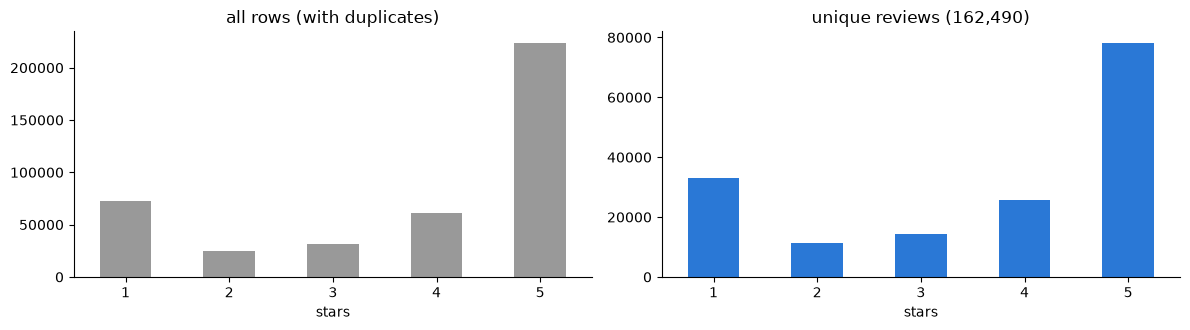
\includegraphics[width=0.95\textwidth]{EC_ratings.png}
\caption{EC: ratings of all rows and of the 162{,}490 unique reviews (before removing 3 stars). People mostly write when
very happy (5) or very unhappy (1); duplicates inflate the 5-star count most.}
\end{figure}

\begin{figure}[H]
\centering
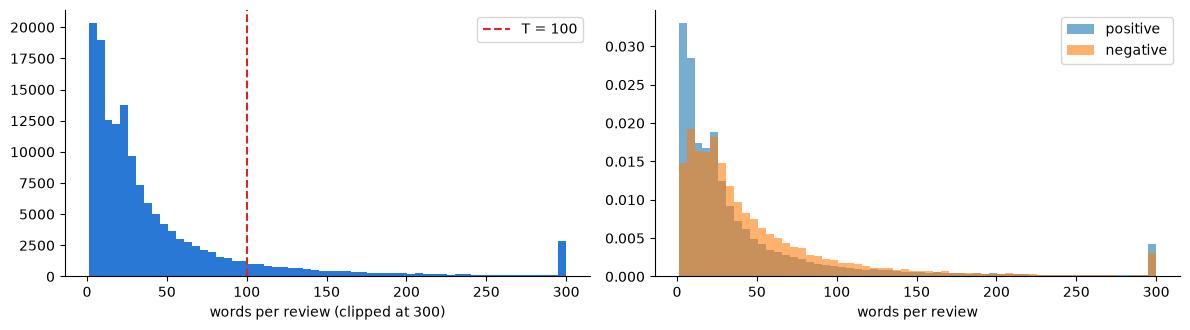
\includegraphics[width=0.95\textwidth]{EC_length.png}
\caption{EC: review length. Negative reviews are longer (median 31 words against 21; 75th percentile 62 against 46);
88.8\,\% of reviews have at most 100 words.}
\end{figure}

\textbf{From text to numbers.} Each review is lower-cased and split into words, each word is replaced by its rank in a
vocabulary of the 20{,}000 most frequent \emph{training} words (id 1 = unknown, 0 = padding), and the sequence is cut or
pre-padded to 100 ids:
\begin{quote}\small
``The bad thing it's too slow even when I have I connected to WiFi\dots'' $\to$ [the, bad, thing, it's, too, slow, \dots]
$\to$ [2, 171, 159, 46, 131, 305, \dots] $\to$ [0, 0, \dots, 0, 2790, 106, 7, 23, 6, 19, 46, 15] (length 100).
\end{quote}
\why{} The vocabulary is built from training reviews only, so no test word influences the model. 20{,}000 of the
54{,}188 distinct words cover 99.3\,\% of all word occurrences (unknown words: 0.73\,\% of tokens). 100 words cover 88.8\,\%
of reviews completely. \emph{Pre}-padding puts the real words at the end of the sequence, next to $h_T$, where the RNN's
memory is strongest.

\begin{figure}[H]
\centering
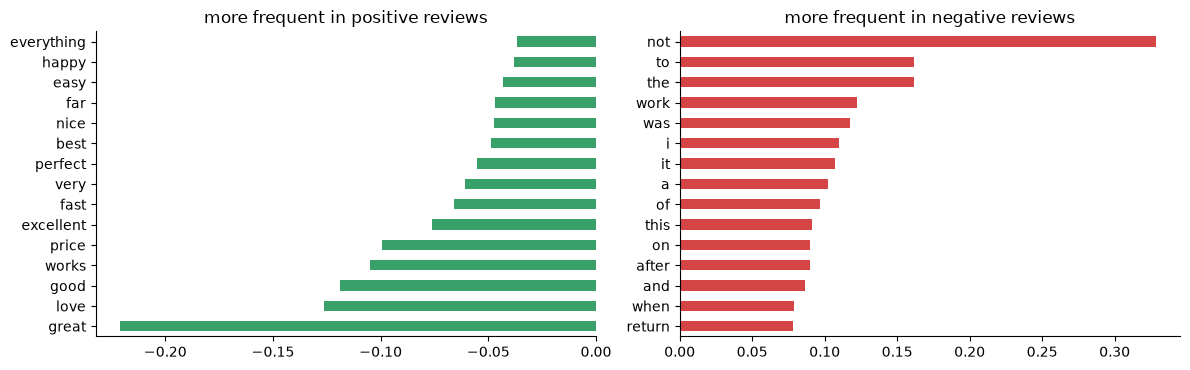
\includegraphics[width=0.95\textwidth]{EC_vocab.png}
\caption{EC: words whose share differs most between classes. Positive reviews use single strong words (``great'', ``love'');
the strongest negative marker is ``not'', whose meaning depends on the next words.}
\label{fig:vocab}
\end{figure}

\subsection{ST: S\&P 500 daily stocks}

Only the 145 stocks with all 3{,}768 trading days are kept, so every stock covers the same dates. Per stock and day:
log return $r_t=\ln(P_t/P_{t-1})$ on the adjusted close, high--low range $(\text{High}-\text{Low})/\text{Close}$, open--close
return $\ln(\text{Close}/\text{Open})$ and log volume. Example: $P$ from 100 to 102 gives $r=\ln1.02=0.0198$. The target is
tomorrow's absolute return $y_t=|r_{t+1}|$, the size of the move. Windows of $T=60$ days (about three months) give 373{,}665 /
81{,}925 / 81{,}925 windows for train (2010--06/2020), validation (to 09/2022) and test (to 12/2024).

\why{}
\emph{Volatility, not direction.} The autocorrelation of returns at lag 1 is $-0.040$: direction is essentially
unpredictable. The autocorrelation of $|r|$ is $0.215$ at lag 1 and still $0.048$ at lag 60 (Figure~\ref{fig:clust}):
large moves cluster, so the size of tomorrow's move is partly predictable from the recent past, which is a real task for a
sequence model. \emph{Chronological split}: a random split would let the model see the future of the test period.
\emph{Scaling} uses train-period statistics only, for the same reason.

\begin{figure}[H]
\centering
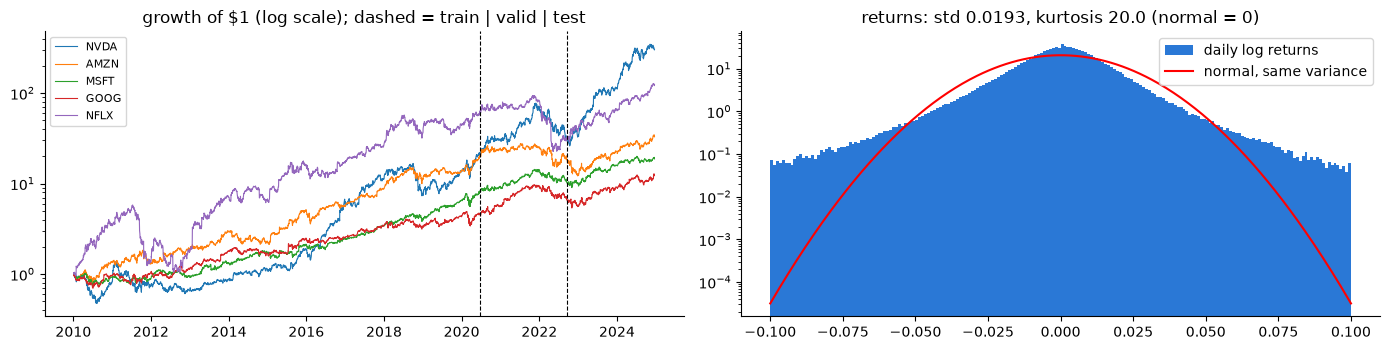
\includegraphics[width=\textwidth]{ST_eda.png}
\caption{ST: normalised prices of five stocks and the distribution of daily returns, which has fat tails.}
\end{figure}

\begin{figure}[H]
\centering
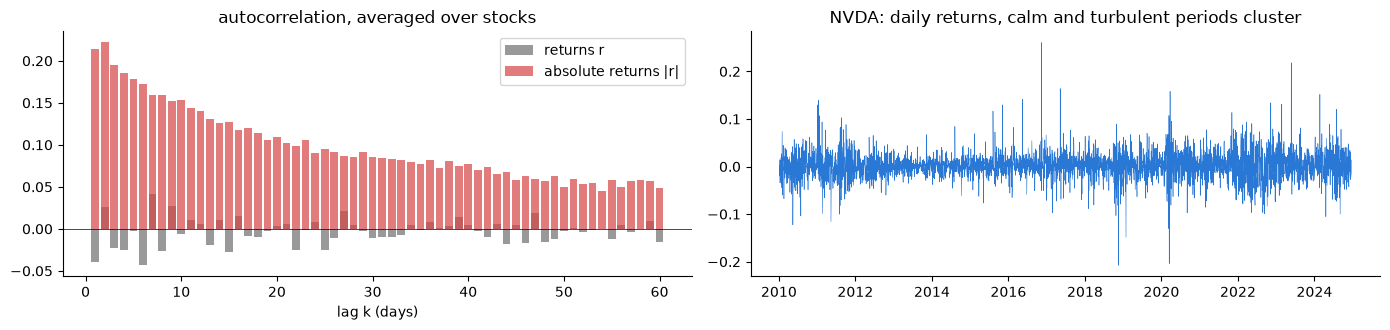
\includegraphics[width=\textwidth]{ST_clustering.png}
\caption{ST: autocorrelation of $r$ (none) and of $|r|$ (positive, decaying over weeks): volatility clustering.}
\label{fig:clust}
\end{figure}

% =====================================================================
\section{Implementation in PyTorch and Keras}
\label{sec:impl}
% =====================================================================

\subsection{The same network in two frameworks}

Keras writes the stack as a list of layers; every layer except the last returns the whole sequence, and the last returns
$h^{(5)}_T$. PyTorch has one module with \texttt{num\_layers=5} that returns the top layer's states for all steps, from
which the forward pass takes the last one. The EC code (ST differs only in the input and the loss):

\begin{lstlisting}[language=Python, title={Keras}]
cell = {"RNN": layers.SimpleRNN, "LSTM": layers.LSTM}[kind]
stack = [layers.Input((MAXLEN,), dtype="int32"), layers.Embedding(VOCAB, EMB)]
stack += [cell(H, return_sequences=(l < LAYERS - 1)) for l in range(LAYERS)]   # layers 1-4: all steps; 5: last
stack += [layers.Dense(1, activation="sigmoid")]                                # g = sigmoid
model = keras.Sequential(stack)
model.compile(optimizer=keras.optimizers.Adam(LR, clipnorm=CLIP), loss="binary_crossentropy")
\end{lstlisting}

\begin{lstlisting}[language=Python, title={PyTorch}]
class TorchSentiment(nn.Module):
    def __init__(self, kind):
        super().__init__()
        self.emb  = nn.Embedding(VOCAB, EMB)
        self.rnn  = {"RNN": nn.RNN, "LSTM": nn.LSTM}[kind](EMB, H, num_layers=LAYERS, batch_first=True)
        self.head = nn.Linear(H, 1)
    def forward(self, x):                        # x: (B, T) word ids
        out, _ = self.rnn(self.emb(x))           # out: (B, T, H), top-layer states
        return self.head(out[:, -1]).squeeze(1)  # logit from h^(5)_T; sigmoid inside BCEWithLogitsLoss
\end{lstlisting}

\subsection{Weight names and verification}

\begin{table}[H]
\centering
\caption{The same weights under three names.}
\small
\begin{tabular}{lll}
\toprule
This report & Keras & PyTorch \\
\midrule
$W_x$ ($F\times H$, or $F\times4H$) & \texttt{kernel} & \texttt{weight\_ih\_l\{k\}}, stored transposed \\
$W_h$ ($H\times H$, or $H\times4H$) & \texttt{recurrent\_kernel} & \texttt{weight\_hh\_l\{k\}}, transposed \\
$b$ & \texttt{bias} & \texttt{bias\_ih\_l\{k\}} + \texttt{bias\_hh\_l\{k\}} \\
gate order & i, f, c, o & i, f, g, o \\
\bottomrule
\end{tabular}
\end{table}

To check that both frameworks compute the compositions of \S3--\S4, the concepts notebook takes the weights of a PyTorch
5-layer network ($F=3$, $H=4$, $T=6$, batch 2), copies them into a NumPy implementation written directly from the
equations and into a Keras stack, and compares the top-layer states:

\begin{table}[H]
\centering
\caption{Maximum absolute difference of $h^{(5)}_t$ over all steps and sequences (float32).}
\small
\begin{tabular}{lrr}
\toprule
 & hand vs PyTorch & hand vs Keras \\
\midrule
5-layer RNN & $6.8\cdot10^{-8}$ & $1.9\cdot10^{-7}$ \\
5-layer LSTM & $3.6\cdot10^{-8}$ & $8.9\cdot10^{-8}$ \\
\bottomrule
\end{tabular}
\end{table}

The differences are at float32 rounding level, so the frameworks compute exactly the functions written above.

\subsection{Identical initialisation}

Both frameworks start from the same distribution: Xavier-uniform input weights, orthogonal recurrent weights, zero biases,
forget-gate bias 1 for the LSTM, embedding uniform in $\pm0.05$. PyTorch's defaults differ (uniform $\pm1/\sqrt H$, forget
bias 0), so the PyTorch models are re-initialised block by block (each of the four gates separately).
\why{} Initialisation decides how much gradient flows at the start (Figure~\ref{fig:grad}); with different defaults a
difference between frameworks could be mistaken for a difference between architectures.

% =====================================================================
\section{Experimental Setup}
\label{sec:setup}
% =====================================================================

\begin{table}[H]
\centering
\caption{One protocol for all 8 runs.}
\small
\begin{tabular}{lll}
\toprule
Setting & EC & ST \\
\midrule
layers / hidden units $H$ & 5 / 64 & 5 / 32 \\
sequence length $T$ & 100 words & 60 days \\
input & embedding $20{,}000\times64$ & 4 z-scored features \\
loss & binary cross-entropy & mean squared error (standardised target) \\
optimizer & \multicolumn{2}{l}{Adam, learning rate $10^{-3}$, gradient clip-norm 1, batch 256} \\
stopping & \multicolumn{2}{l}{at most 10 epochs; early stopping on validation loss, patience 2, best weights restored} \\
seed & \multicolumn{2}{l}{42 for Python, NumPy, TensorFlow and PyTorch} \\
\bottomrule
\end{tabular}
\end{table}

\textbf{Baselines.} EC: the \emph{majority class} (always positive), the floor; and \emph{TF-IDF + logistic regression},
a strong classical model that ignores word order, to show what word order is worth. ST: the \emph{train mean} (the zero of
$R^2_{\text{oos}}$), \emph{persistence} $\hat y=|r_t|$, and the \emph{20-day mean} of $|r|$, the classical volatility estimate,
which shows what simply averaging the recent past gives.

\textbf{Metrics.} EC: accuracy, macro F1 (the mean of the two classes' F1, so the 30\,\% negative class counts as much as
the positive one), F1 of the negative class (the reviews a shop most needs to catch) and ROC-AUC (ranking quality,
independent of the 0.5 threshold). ST: RMSE and MAE in percent of daily move,
$R^2_{\text{oos}}=1-\sum(y-\hat y)^2/\sum(y-\bar y_{\text{train}})^2$ and the correlation of forecast and truth.

\textbf{Machine.} The dataset notebooks were run on a Windows PC on CPU (TensorFlow 2.22.0-rc0, PyTorch 2.14.1+cpu).
Times compare models on this machine only.

% =====================================================================
\section{Results: EC Review Sentiment}
\label{sec:ec}
% =====================================================================

\begin{table}[H]
\centering
\caption{EC test set (22{,}219 reviews). Bold: best network.}
\label{tab:ec}
\small
\resizebox{\textwidth}{!}{\begin{tabular}{lrrrrrrr}
\toprule
Run & Accuracy & F1 macro & F1 neg. & ROC-AUC & Params & s/epoch & Epochs (best) \\
\midrule
\textit{majority class} & 0.7006 & 0.4120 & 0.0000 & 0.5000 & -- & -- & -- \\
\textit{TF-IDF + log. regression} & 0.9414 & 0.9298 & 0.9011 & 0.9825 & -- & -- & -- \\
\midrule
\run{EC-TF-RNN} & 0.9225 & 0.9084 & 0.8726 & 0.9707 & 1{,}321{,}345 & 53 & 4 (2) \\
\run{EC-TF-LSTM} & 0.9301 & 0.9161 & 0.8817 & 0.9745 & 1{,}445{,}185 & 256 & 4 (2) \\
\run{EC-PT-RNN} & 0.9183 & 0.8999 & 0.8570 & 0.9676 & 1{,}321{,}665 & 58 & 4 (2) \\
\run{EC-PT-LSTM} & \textbf{0.9311} & \textbf{0.9176} & \textbf{0.8844} & \textbf{0.9760} & 1{,}446{,}465 & 143 & 5 (3) \\
\bottomrule
\end{tabular}
}
\end{table}

\begin{figure}[H]
\centering
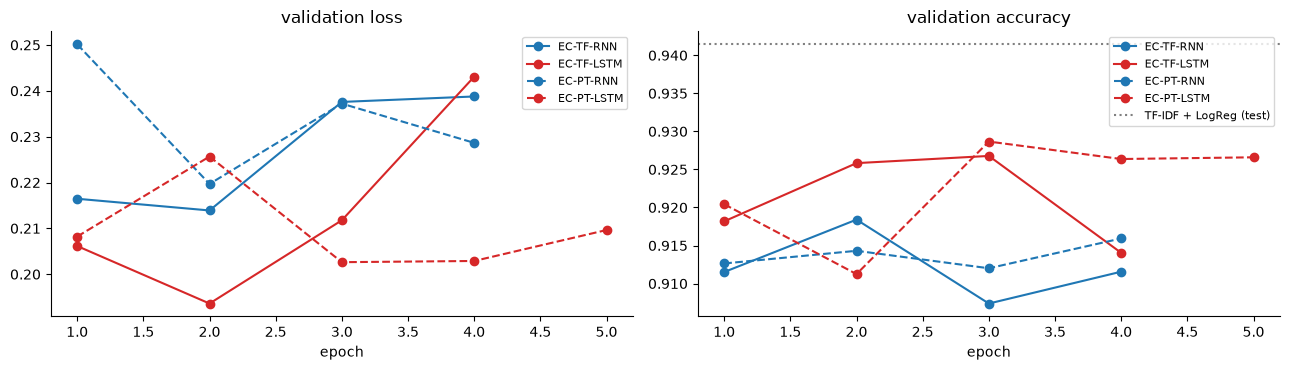
\includegraphics[width=\textwidth]{EC_curves.png}
\caption{EC: validation loss and accuracy per epoch (solid = Keras, dashed = PyTorch; blue = RNN, red = LSTM).}
\label{fig:eccurves}
\end{figure}

\textbf{The LSTM beats the RNN in both frameworks}: accuracy 0.930/0.931 against 0.922/0.918, negative-class F1
0.882/0.884 against 0.873/0.857, and the best validation loss of each LSTM is lower than that of the RNN in the same
framework (0.194 against 0.214 in Keras, 0.203 against 0.220 in PyTorch; Figure~\ref{fig:eccurves}).
\why{} Negative reviews are longer and explain what went wrong over many words, and the strongest negative marker,
``not'', only means something together with the words that follow (Figure~\ref{fig:vocab}). Holding such information
until the end of the sequence is exactly what the additive cell makes trainable (\S\ref{sec:lstm}).

\begin{table}[H]
\centering
\caption{EC: test accuracy by review length (words before cutting to 100). LSTM $-$ RNN averaged over the two frameworks.}
\label{tab:eclen}
\small
\begin{tabular}{lrrrrrr}
\toprule
Words & \run{EC-TF-RNN} & \run{EC-TF-LSTM} & \run{EC-PT-RNN} & \run{EC-PT-LSTM} & LSTM $-$ RNN & Reviews \\
\midrule
1--10 & 0.950 & 0.952 & 0.945 & 0.954 & +0.006 & 5{,}955 \\
11--20 & 0.929 & 0.936 & 0.920 & 0.938 & +0.013 & 3{,}697 \\
21--40 & 0.926 & 0.937 & 0.926 & 0.936 & +0.011 & 5{,}546 \\
41--70 & 0.914 & 0.925 & 0.907 & 0.923 & +0.014 & 3{,}070 \\
71--100 & 0.911 & 0.919 & 0.907 & 0.918 & +0.010 & 1{,}458 \\
$>$100 (cut) & 0.855 & 0.868 & 0.855 & 0.874 & +0.016 & 2{,}493 \\
\bottomrule
\end{tabular}

\end{table}

\begin{figure}[H]
\centering
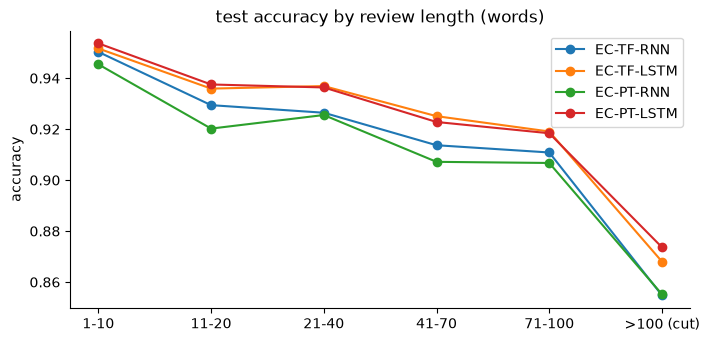
\includegraphics[width=0.62\textwidth]{EC_by_length.png}
\caption{EC: accuracy by review length.}
\end{figure}

\textbf{Accuracy falls with length for every model, and the LSTM's lead grows} from $+0.006$ on reviews of 1--10 words to
$+0.016$ on reviews longer than 100 words (Table~\ref{tab:eclen}).
\why{} Short reviews (``Great phone!'') are decided by one word near the end, which any model reads. Long reviews mix
praise and complaints, and the decisive part may be far from the last step; the RNN's gradient from those words has
vanished, the LSTM's has not. Reviews longer than 100 words are hardest for all models because the cut removes their end,
which is often where the verdict is.

\textbf{Overfitting starts after 2--3 epochs.} Training loss keeps falling (to 0.09 for \run{EC-PT-LSTM}) while validation
loss rises after epoch 2 or 3, and early stopping keeps the best epoch.
\why{} 89--97\,\% of the parameters (1.28\,M) are in the embedding, learned from scratch on 104\,k reviews; rare words get
memorised quickly.

\begin{figure}[H]
\centering
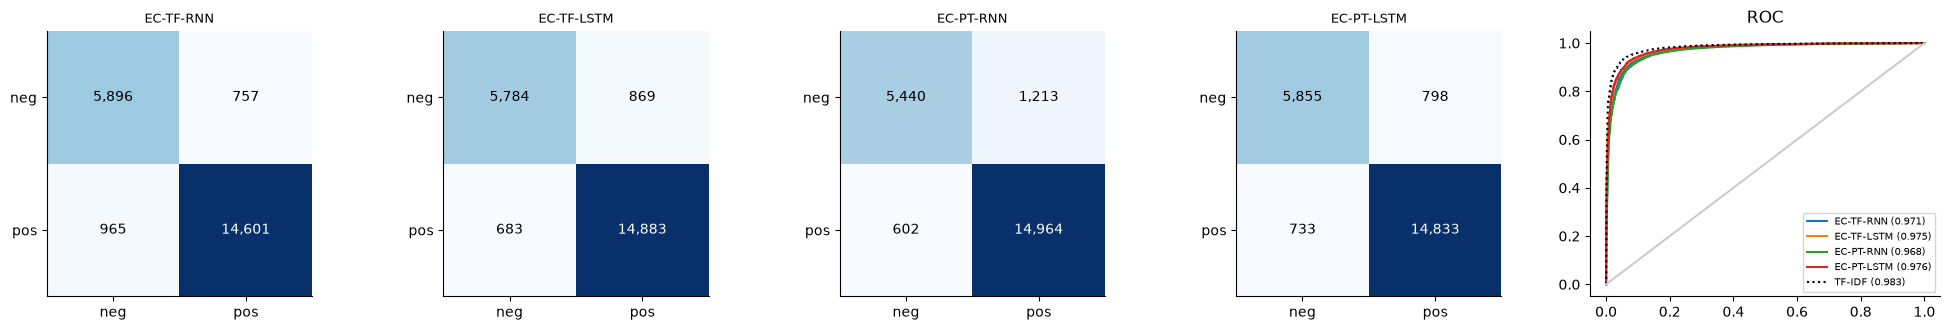
\includegraphics[width=\textwidth]{EC_confusion_roc.png}
\caption{EC: confusion matrices (rows = true class) and ROC curves.}
\end{figure}

\textbf{TF-IDF + logistic regression is better than both networks} (accuracy 0.941, macro F1 0.930, AUC 0.983), a negative
result that we report as measured.
\why{} In these reviews sentiment is carried mostly by single words (``great'', ``love'', ``return'', ``broke''), which a
bag-of-words model sees directly, for every word of every review, with a convex training problem. The networks see at most
100 words, must learn 1.28\,M embedding weights from scratch from 104\,k examples, and stop after 2--3 useful epochs. Word
order helps (the LSTM beats the RNN), but not enough to make up for this. Pretrained embeddings or a bidirectional LSTM
would be the next step (\S\ref{sec:limits}).

\textbf{Where the two architectures disagree.} The Keras RNN and LSTM disagree on 782 of 22{,}219 test reviews. Typical cases:

\begin{table}[H]
\centering
\caption{EC: test reviews scored by \run{EC-TF-RNN} and \run{EC-TF-LSTM} ($P$ = probability of positive).}
\small
\begin{tabularx}{\textwidth}{Xrrr}
\toprule
Review (start) & Stars & $P$ RNN & $P$ LSTM \\
\midrule
``Love the phone, but it drains the battery fairly quickly. Very slick, therefore easy to lose grip\dots'' & 4 & 0.494 & 0.834 \\
``I think it was a good phone but my teenage son\dots broke it after having it only two weeks.'' & 4 & 0.287 & 0.534 \\
``\dots there is not problem with this jet.'' & 5 & 0.360 & 0.547 \\
``I ordered a brand new samsung galaxy s4\dots the phone delivered to me is `used' one\dots I am very disappointed\dots'' & 1 & 0.669 & 0.378 \\
``I'm changing my review from 4 stars to 2. This Deluxe Edition 128gb does not work with U.S. carriers\dots'' & 2 & 0.437 & 0.649 \\
\bottomrule
\end{tabularx}
\end{table}

The first three are mixed reviews whose positive verdict comes early (``Love the phone'', ``good phone'') or is negated
(``not problem''); the RNN is swayed by the complaint words near the end, the LSTM keeps the earlier verdict.
The fourth is a negative review that starts with neutral product details; the LSTM gets it right. The last one is an LSTM
error: a 2-star review that opens with ``4 stars'' and a neutral product description; the early, positive-sounding
content probably outweighs the complaint that follows.

% =====================================================================
\section{Results: ST Stock Volatility}
\label{sec:st}
% =====================================================================

\begin{table}[H]
\centering
\caption{ST test period (09/2022--12/2024, 81{,}925 windows). Errors in percent of daily move. Bold: best network.}
\label{tab:st}
\small
\resizebox{\textwidth}{!}{\begin{tabular}{lrrrrrrr}
\toprule
Run & RMSE (\%) & MAE (\%) & $R^2_{\text{oos}}$ & Corr. & Params & s/epoch & Epochs (best) \\
\midrule
\textit{train mean} & 1.3632 & 0.8809 & 0.0000 & -- & -- & -- & -- \\
\textit{persistence $|r_t|$} & 1.7783 & 1.1281 & -0.7018 & 0.149 & -- & -- & -- \\
\textit{20-day mean $|r|$} & 1.3326 & 0.8656 & 0.0443 & 0.251 & -- & -- & -- \\
\midrule
\run{ST-TF-RNN} & 1.3015 & 0.8419 & 0.0884 & 0.300 & 9{,}537 & 67 & 3 (1) \\
\run{ST-TF-LSTM} & 1.2990 & \textbf{0.8158} & 0.0920 & 0.311 & 38{,}049 & 175 & 6 (4) \\
\run{ST-PT-RNN} & 1.3025 & 0.8238 & 0.0871 & 0.299 & 9{,}697 & 71 & 4 (2) \\
\run{ST-PT-LSTM} & \textbf{1.2957} & 0.8399 & \textbf{0.0965} & 0.311 & 38{,}689 & 127 & 5 (3) \\
\bottomrule
\end{tabular}
}
\end{table}

\textbf{Baselines.} Persistence is far \emph{worse} than the train mean ($R^2_{\text{oos}}=-0.70$), while the 20-day
mean is better ($+0.044$).
\why{} One day's move is a very noisy estimate of tomorrow's: a 5\,\% day is often followed by a 1\,\% day. Averaging
20 days removes most of that noise and keeps the volatility level, which persists (Figure~\ref{fig:clust}).

\textbf{All four networks beat every baseline}, with $R^2_{\text{oos}}$ 0.087--0.096, about twice the 20-day mean, and a
correlation of 0.30--0.31 with the true move.
\why{} A network can weight the recent days adaptively instead of equally, and it also uses the high--low range and volume,
which carry information about volatility that $|r|$ alone does not. $R^2\approx0.1$ is low in absolute terms but normal for
daily volatility: most of tomorrow's move is news that no price history contains.

\textbf{The LSTM is only marginally better than the RNN}: RMSE 1.2957--1.2990 against 1.3015--1.3025, $\Delta R^2$
$+0.004$ (Keras) and $+0.009$ (PyTorch).
\why{} The autocorrelation of $|r|$ falls from 0.215 to below 0.05 within the 60-day window, so the useful information
sits in the last few weeks, which the RNN's gradient can still reach. The LSTM's long memory has little extra to find.

\begin{table}[H]
\centering
\caption{ST: test RMSE (\%) by volatility level at prediction time (quintiles of the 20-day mean of $|r|$).}
\label{tab:regime}
\small
\resizebox{\textwidth}{!}{\begin{tabular}{lrrrrrr}
\toprule
20-day volatility & \run{ST-TF-RNN} & \run{ST-TF-LSTM} & \run{ST-PT-RNN} & \run{ST-PT-LSTM} & 20-day mean & LSTM $-$ RNN \\
\midrule
calmest & 0.9813 & 0.9829 & 0.9839 & 0.9810 & 1.0108 & -0.0006 \\
calm & 1.0622 & 1.0596 & 1.0633 & 1.0617 & 1.0791 & -0.0021 \\
middle & 1.2380 & 1.2354 & 1.2389 & 1.2326 & 1.2525 & -0.0044 \\
turbulent & 1.3154 & 1.3123 & 1.3168 & 1.3098 & 1.3395 & -0.0050 \\
most turbulent & 1.7650 & 1.7605 & 1.7648 & 1.7522 & 1.8248 & -0.0086 \\
\bottomrule
\end{tabular}
}
\end{table}

\textbf{Where the LSTM helps: turbulent periods.} Its advantage grows from $-0.0006$ in the calmest fifth of days to
$-0.0086$ in the most turbulent fifth (Table~\ref{tab:regime}).
\why{} After a shock the model must remember that the market has been turbulent for weeks and decide how fast that will
fade; in calm periods the last few days already say everything.

\begin{figure}[H]
\centering
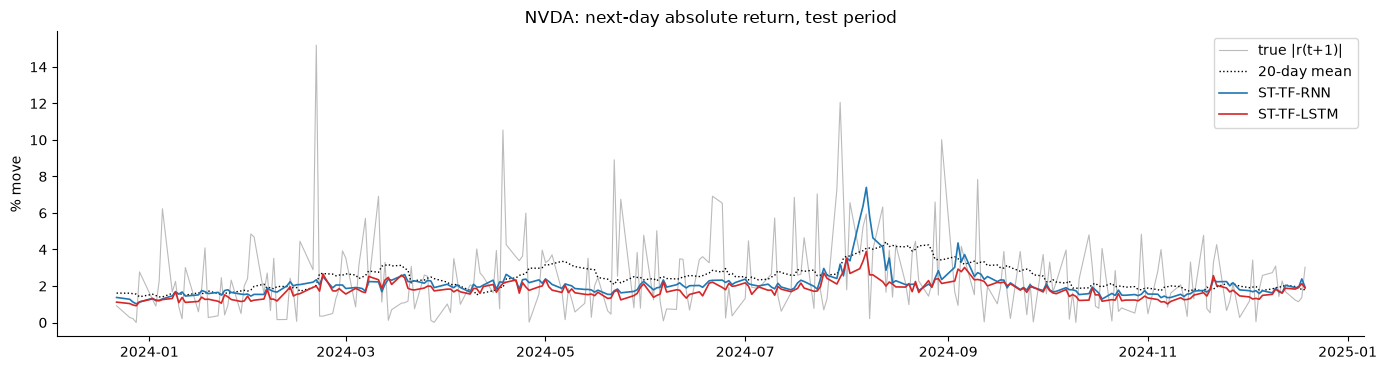
\includegraphics[width=\textwidth]{ST_forecast.png}
\caption{ST: true next-day move of NVDA in the last 250 test days, with the 20-day mean and the Keras forecasts.}
\label{fig:forecast}
\end{figure}

\textbf{The forecasts are smooth and miss the spikes} (Figure~\ref{fig:forecast}).
\why{} With squared-error loss the best forecast is the \emph{conditional mean} of $|r_{t+1}|$. A spike such as the 15\,\%
move in February 2024 is not predictable from prices, so the model forecasts the expected size (about 2\,\%) and rises after
spikes, which is the volatility clustering it has learned.

\begin{figure}[H]
\centering
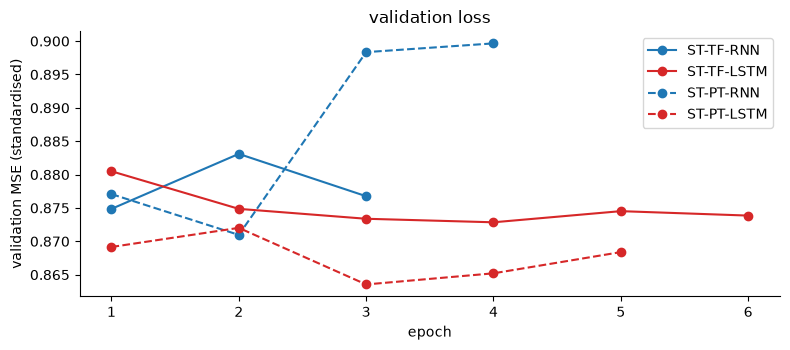
\includegraphics[width=0.62\textwidth]{ST_curves.png}
\caption{ST: validation loss per epoch.}
\end{figure}

\textbf{Training stops early (best epoch 1--4) and validation loss is above training loss} (about 0.87 against 0.74).
\why{} The validation period (mid-2020 to 2022: post-COVID recovery, inflation, rate hikes) is a different market regime
from the training period, so after a few epochs further fitting of the training years no longer transfers.

% =====================================================================
\section{Comparison: RNN against LSTM}
\label{sec:compare}
% =====================================================================

Following the lecturer's comparison criteria (accuracy, parameters, training time and behaviour):

\begin{figure}[H]
\centering
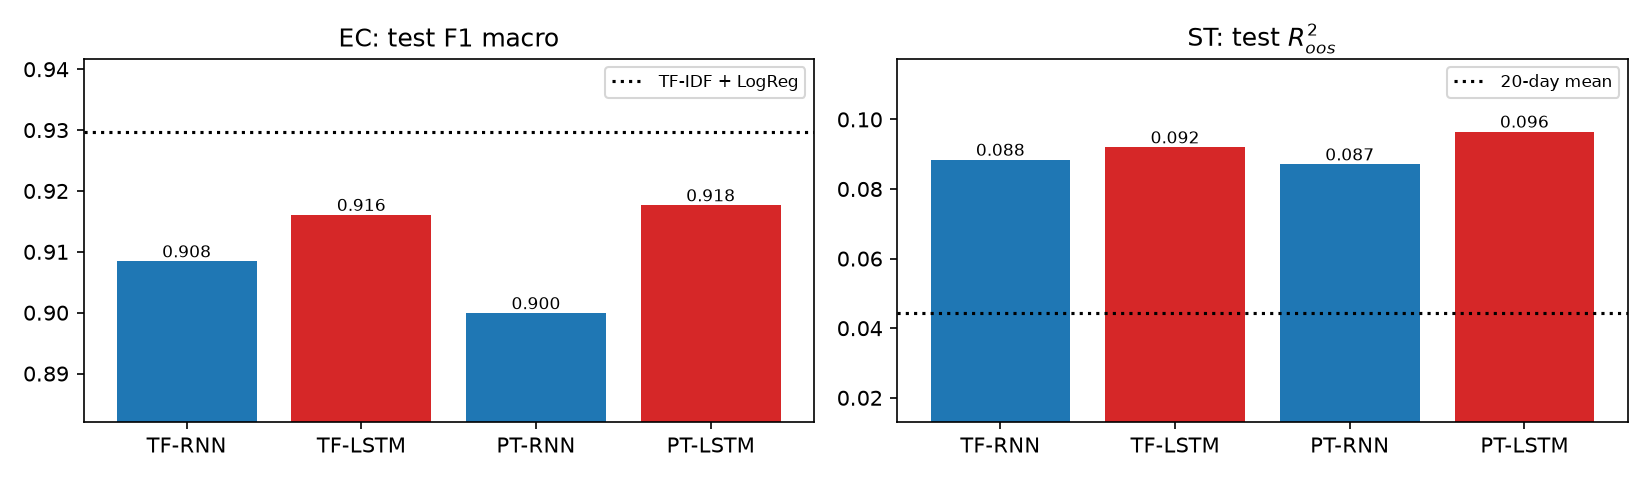
\includegraphics[width=\textwidth]{cmp_score.png}
\caption{Main test score of the 8 runs with the strongest baseline (dotted).}
\end{figure}

\begin{enumerate}
\item \textbf{Accuracy.} The LSTM is better in all four pairs (Table~\ref{tab:summary}). The gain is clear on EC (macro F1
  $+0.008$ / $+0.018$) and small on ST ($R^2$ $+0.004$ / $+0.009$).
  \why{} The size of the gain follows the length of the dependency the task needs: long on EC (verdicts far from the end,
  negation), short on ST (volatility memory of a few weeks).
\item \textbf{Parameters.} The LSTM has 4$\times$ the recurrent weights. On ST that is the whole model (9.5\,k $\to$ 38\,k);
  on EC the shared embedding makes it only $+9\,\%$. The extra parameters buy controlled memory, not capacity of the same
  kind: an RNN with 4$\times$ as many units would still have the multiplicative gradient path.
\item \textbf{Time.} The LSTM takes 1.8--4.8$\times$ longer per epoch (Figure~\ref{fig:time}).
  \why{} Each step computes four gate products instead of one, plus the cell update. The ratio is larger in Keras on EC
  (53 $\to$ 256\,s) than in PyTorch (58 $\to$ 143\,s) because the two frameworks use different CPU kernels for the LSTM.
\item \textbf{Behaviour.} At initialisation the LSTM passes about $5\cdot10^{6}$ times more gradient to the first step
  (Figure~\ref{fig:grad}); after training its advantage concentrates where memory matters: long reviews
  (Table~\ref{tab:eclen}) and turbulent markets (Table~\ref{tab:regime}).
\end{enumerate}

\begin{figure}[H]
\centering
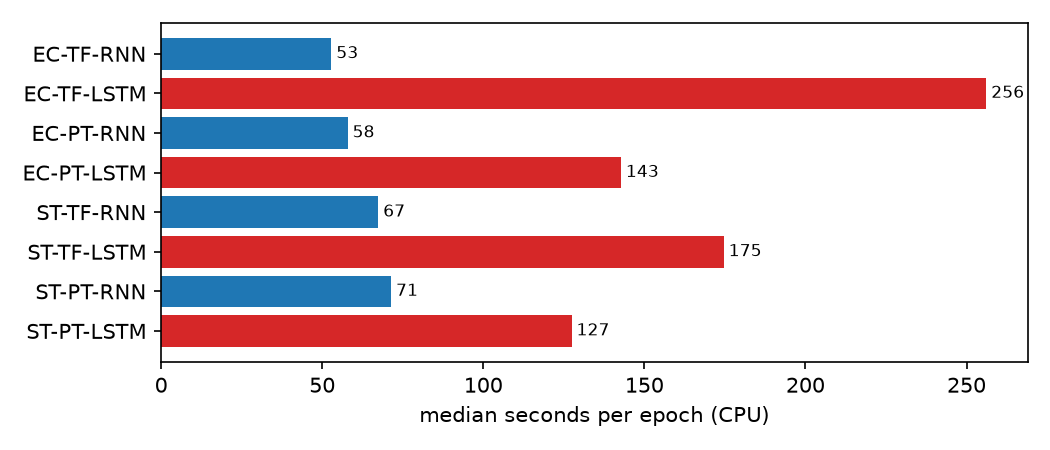
\includegraphics[width=0.62\textwidth]{cmp_time.png}
\caption{Median seconds per epoch on CPU (blue = RNN, red = LSTM).}
\label{fig:time}
\end{figure}

\textbf{Keras against PyTorch.} The two frameworks compute the same function (\S\ref{sec:impl}) and give the same ranking
everywhere; their scores differ by at most 0.016 (negative-class F1 of the EC RNNs).
\why{} The data, architecture, initial distribution and stopping rule are identical, but the actual random weights, the
order of the mini-batches and the floating-point kernels are not, and early stopping then picks a different epoch
(e.g.\ 2 against 3 for the EC LSTMs). The parameter counts differ only by PyTorch's second bias.

% =====================================================================
\section{Limitations}
\label{sec:limits}
% =====================================================================

\begin{itemize}
\item \textbf{One run per configuration.} No repeated seeds, so differences below about 0.005 (e.g.\ the ST RNN--LSTM gap in
  Keras) are within run-to-run noise.
\item \textbf{EC reads at most 100 words}, left to right, with embeddings learned from scratch; pretrained embeddings or a
  bidirectional LSTM would likely close the gap to TF-IDF.
\item \textbf{No tuning per model}: $H$, learning rate and depth are the same for both architectures, so each might do
  better with its own settings.
\item \textbf{ST regime shift}: train, validation and test are different market periods, and only next-day volatility is
  forecast.
\item \textbf{CPU timing} on one machine; on a GPU with cuDNN the time ratio would differ.
\end{itemize}

% =====================================================================
\section{Conclusion}
% =====================================================================

Written as compositions of matrix product, addition, $\tanh$, sigmoid and element-wise product, the 5-layer RNN and LSTM
differ in one mechanism: the LSTM's additive, gated cell. The chain rule shows why it matters (the RNN's gradient is a
product of shrinking factors, the LSTM's cell gradient is a product of forget gates), and the measured gradient maps
confirm it ($8.7\cdot10^{-11}$ against $4.5\cdot10^{-4}$ at the first step). PyTorch and Keras compute exactly these
compositions, with hand-counted parameters.

On real data the mechanism pays off in proportion to how far back the needed information lies. On e-commerce reviews the
LSTM is clearly better than the RNN and most so on long reviews, although a bag-of-words baseline is still better than
both. On stock volatility both networks double the classical 20-day estimate and the LSTM adds little, except in turbulent
periods. The LSTM costs 4$\times$ the recurrent parameters and up to 4.8$\times$ the time, so it is worth choosing when the
task has long-range dependencies (EC) and is optional when the signal is recent (ST).

% =====================================================================
\appendix
\section{Reproducibility}
\label{app:repro}
% =====================================================================

\begin{tabularx}{\textwidth}{lX}
\toprule
Path & Content \\
\midrule
\texttt{dataset/README.md} & Kaggle links and download commands (raw files are not committed) \\
\texttt{notebook/00\_rnn\_lstm\_concepts.ipynb} & elementary functions, 5-layer RNN and LSTM by hand, checks against PyTorch and Keras, parameters, gradient maps \\
\texttt{notebook/ec\_reviews.ipynb} & EC: cleaning, tokenisation, baselines, 4 runs, evaluation \\
\texttt{notebook/st\_stocks.ipynb} & ST: features, windows, baselines, 4 runs, evaluation \\
\texttt{notebook/results/} & one JSON per run, \texttt{EC\_comparison.csv}, \texttt{ST\_comparison.csv} \\
\texttt{report/extract\_figures.py} & saves the concepts and EC exploration figures from the executed notebooks \\
\texttt{report/make\_tables.py} & writes \texttt{table\_*.tex} and the comparison charts from \texttt{results/} \\
\texttt{requirements.txt} & Python packages (Python 3.10--3.12) \\
\bottomrule
\end{tabularx}

Run order: download the data; run the three notebooks; \texttt{python report/extract\_figures.py};
\texttt{python report/make\_tables.py}; \texttt{xelatex Assignment\_07.tex} twice in \texttt{report/}.

\end{document}
